\documentclass[18pt]{beamer}
\usepackage[utf8]{inputenc} % for the umlauts
\usepackage{subfigure}

\beamertemplatenavigationsymbolsempty
%% SLIDE FORMAT

% use 'beamerthemekit' for standard 4:3 ratio
% for widescreen slides (16:9), use 'beamerthemekitwide'

\usepackage{templates/beamerthemekit}
% \usepackage{templates/beamerthemekitwide}

\setcounter{tocdepth}{1}

%% TITLE PICTURE

% if a custom picture is to be used on the title page, copy it into the 'logos'
% directory, in the line below, replace 'mypicture' with the 
% filename (without extension) and uncomment the following line
% (picture proportions: 63 : 20 for standard, 169 : 40 for wide
% *.eps format if you use latex+dvips+ps2pdf, 
% *.jpg/*.png/*.pdf if you use pdflatex)

%\titleimage{mypicture}

%% TikZ INTEGRATION

% use these packages for PCM symbols and UML classes
% \usepackage{templates/tikzkit}
% \usepackage{templates/tikzuml}

% the presentation starts here

\usepackage[absolute,overlay]{textpos}
%\usepackage[texcoord,grid,gridunit=mm,gridcolor=red, subgridcolor=green]{eso-pic}
\setbeamercovered{invisible}

\title[SWT1]{Softwaretechnik 1 - 2. Tutorium}
\subtitle{Tutorium 03}
\author{Felix Bachmann}
\date{29.05.2017}

\institute{KIT - Institut für Programmstrukturen und Datenorganisation (IPD)}

% Bibliography

\usepackage[citestyle=authoryear,bibstyle=numeric,hyperref,backend=biber]{biblatex}
\addbibresource{templates/example.bib}
\bibhang1em

\begin{document}

% change the following line to "ngerman" for German style date and logos
\selectlanguage{ngerman}

%title page
\begin{frame}
\titlepage
\end{frame}

%table of contents
\begin{frame}{Themenübersicht}
\tableofcontents
\end{frame}

\section{Orga}
	\subsection{Feedback 2. Übungsblatt}
	\begin{frame}
		\frametitle{2. Übungsblatt Statistik}
		%TODO add statistics chart [scale=0.7]{./pics/tut2/statistics_ub1.png}
	\end{frame}
	
	\subsection{2. Übungsblatt - Fehler (Allgemein)}
	\begin{frame}
		\frametitle{Häufige Fehler}
		\begin{block}{Allgemein}
			%TODO add common faults
		\end{block}
	\end{frame}
	
	\subsection{2. Übungsblatt - Fehler}
	\begin{frame}
		\frametitle{Häufige Fehler}
		\begin{block}{Aufgabe 1 (??)}
			%TODO add exercise specific faults
		\end{block}
	\end{frame}

\section{Main}
		
\section{Tipps}
	\subsection{Tipps}
	\begin{frame}
		\frametitle{Tipps - 3. Übungsblatt}
		\begin{small}
			\begin{exampleblock}{Aufgabe 1-3: Plug-In programmieren}
				\begin{itemize}
					\item l%TODO tipps? allgemein javadoc etc.? [abhängig von UB 2]
				\end{itemize}
			\end{exampleblock}
			\pause
			\begin{exampleblock}{Aufgabe 4: Aktivitätsdiagramm}
				\begin{itemize}
					\item l%TODO tipps
				\end{itemize}
			\end{exampleblock}
			\pause
			\begin{exampleblock}{Aufgabe 5: Sequenzdiagramm}
				\begin{itemize}
					\item l%TODO tipps
				\end{itemize}
			\end{exampleblock}
		\end{small}
	\end{frame}
	
	\subsection{Abgabe}
	\begin{frame}
		\frametitle{Denkt dran!}
		\begin{alertblock}{Abgabe}
			\begin{itemize}
				\item Deadline am 7.6 um 12:00
				\item Aufgabe 4+5 handschriftlich (auf saubere Syntax achten!)
			\end{itemize}
		\end{alertblock}
	\end{frame}
		
	\begin{frame}
		\frametitle{Bis dann! (dann := 12.06.17)}
		\centering
		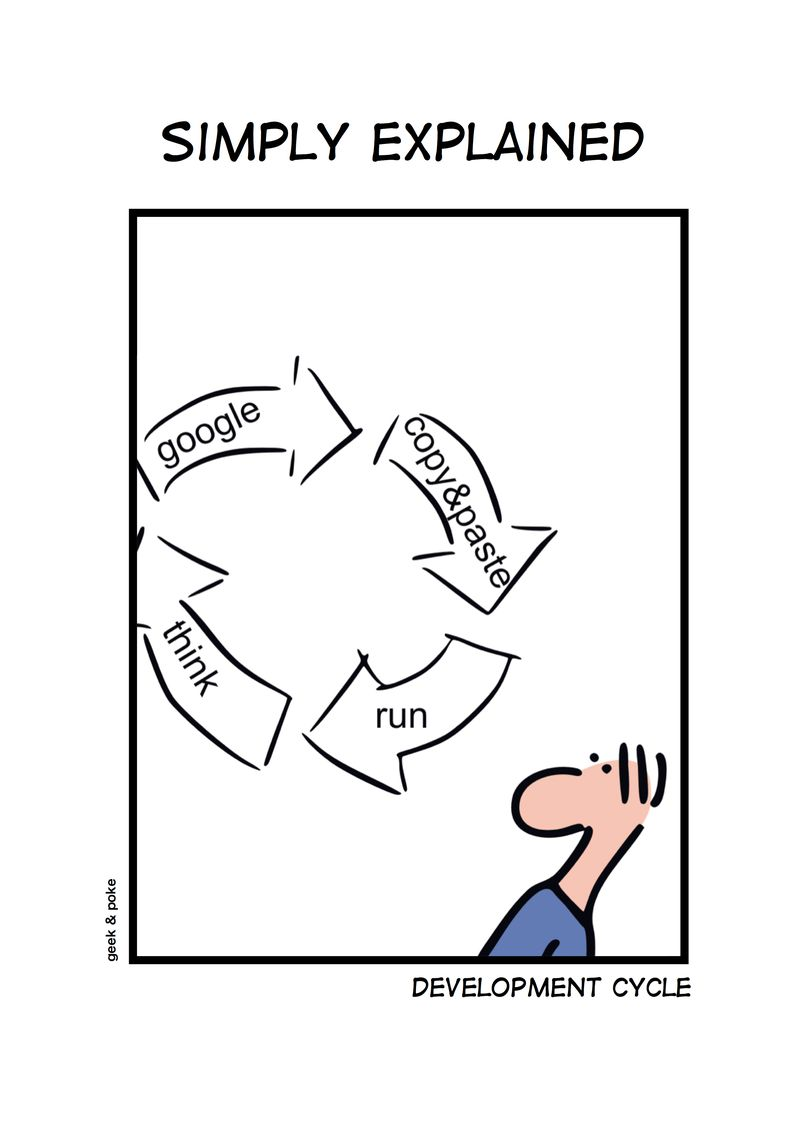
\includegraphics[scale=0.9]{./comics/geek_and_poke_development.jpg}
	\end{frame}

\end{document}
